\documentclass{article}
\usepackage[utf8]{inputenc}
\usepackage[spanish]{babel}
\usepackage[hidelinks]{hyperref}
\usepackage{setspace}
\usepackage{graphicx}
\usepackage{float}
\usepackage[hidelinks]{hyperref}
\usepackage{dirtree}
\usepackage{pdflscape}
\usepackage{pdfpages}


\usepackage[compact]{titlesec}
\usepackage{geometry}
\geometry{
    a4paper,
    total={170mm,257mm},
    left=30mm, % entre 25-35
    right=30mm, % entre 25-35
    top=30mm, % no más de 30
    bottom=25mm, % no más de 30
}

\usepackage{fancyhdr}
\pagestyle{fancy}
\fancyhf{}
\lhead{}
\rhead{Bárbaros Software S.A.}
\rfoot{\thepage}
\lfoot{Plan de gestión, análisis, diseño y memorial del proyecto KeyPaX}
\renewcommand{\footrulewidth}{0.4pt}

\setlength{\parindent}{2em}
\setlength{\parskip}{1em}

\begin{document}

\begin{titlepage}
    \centering
    \vspace*{\fill}

    \vspace*{0.5cm}

    \Huge
    \textbf{Plan de gestión, análisis, diseño y memorial del proyecto KeyPaX}

    \vspace*{0.5cm}

    \huge
    Bárbaros Software S.A. (Grupo 3)

    
\includegraphics[height=5cm,angle=-45]{../images/llave.png}

    \begin{Large}
        Carlos Bellvis, 755452\\
        Jorge Bernal, 775695\\
        Jorge Borque, 777959\\
        Arturo Calvera, 776303\\
        Andoni Salcedo, 785649\\
        Javier Vela, 775593\\
    \end{Large}

    \vspace*{1cm}

    \large
    \href{https://github.com/UNIZAR-30226-2021-03}{Organización GitHub: https://github.com/UNIZAR-30226-2021-03}

    \vspace*{\fill}

\end{titlepage}

\pagebreak

\tableofcontents

\pagebreak

\section{Introducción}

En el siguiente documento se presenta el sistema KeyPaX, va a ser desarrollado por Bárbaros Software S.A. y permite gestionar contraseñas almacenadas remotamente en los servidores del sistema. Permite almacenar junto con las contraseñas el nombre de usuario, URL y una descripción textual, entre otros. Las contraseñas se pueden organizar por categorías para subdividir las contraseñas por temática.

Además, para mejorar la seguridad del sistema, se podrán generar automáticamente contraseñas robustas con longitud y caracteres variables. El usuario accederá al servicio mediante una contraseña maestra y deberá identificarse en el inicio de sesión mediante el 2FA.

Para acceder al sistema se utilizará la aplicación para móviles Android o en navegador web. Se utilizará Java (Android SDK) y JavaScript (React.JS), respectivamente, para implementar las vistas del sistema. El \textit{backend} se desarrollará utilizando Node.JS y la \textit{framework} Express. Por último, la base de datos utilizará el SGBD MongoDB. 

El despliegue del sistema se realizará en un entorno de contenedores Docker. Mediante Docker se puede aprovechar al máximo los recursos \textit{hardware} de la máquina, aumentando la portabilidad del sistema y ahorrando en fallos de desarrollo. 

Se plantea un plan de trabajo, dónde se comprometen varias fechas para las entregas anteriores a la finalización del proyecto.  El día 15 de abril de 2021 se entregará una primera versión del sistema \textit{software}. Tras las modificaciones y correcciones propuestas por el cliente, el 21 de mayo de 2021 se presentará una segunda versión. El 1 de junio de 2021, Bárbaros Software S.A. se compromete a entregar el sistema final al cliente.

En el documento se estipulan los procesos y planes a llevar por los integrantes del proyecto al desarrollar el producto. Estos planes son precisos para llevar un análisis de calidad adecuado y para la organización de directorios del proyecto, entre otros.

Se presentan los requisitos de manera precisa y sin ambigüedades, especificando exactamente la funcionalidad del sistema. Además, se presentan varias vistas del sistema en forma de diagramas de despliegue, componentes y módulos.

Por último, se realiza una memoria del trabajo, comentando el desarrollo del proyecto y del producto. En la memoria se profundiza en la ejecución de los planes, procesos y organización propuesta, sus problemas y su resultado. 

\pagebreak


\section{Organización del proyecto}

El equipo del proyecto está formado por los 6 integrantes del grupo.  Para dividir el trabajo y las responsabilidades se han formado 2 grupos iniciales,  de acuerdo con las capacidades y conocimientos individuales.  Además, se ha designado como director del proyecto a Arturo Calvera, sobre el cual recae la gestión de los equipos de trabajo y de las responsabilidades de los mismos.

\begin{itemize}
    \setlength{\itemsep}{0em}
    \item \textbf{Director del proyecto}: Arturo Calvera
    \begin{itemize}
        \setlength{\itemsep}{0em}
        \item Función: Planificación y organización del equipo. Responsable de que se cumplan las tareas designadas.
    \end{itemize}
    \item \textbf{Equipo \textit{Backend}}:
    \begin{itemize}
        \setlength{\itemsep}{0em}
        \item Responsable: Arturo Calvera.
        \item Función: Desarrollo del \textit{backend} del sistema.
        \item Integrantes: Arturo Calvera, Andoni Salcedo.
    \end{itemize}
    \item \textbf{Equipo \textit{Frontend}}:
    \begin{itemize}
        \setlength{\itemsep}{0em}
        \item Responsable: Javier Vela.
        \item Sub-equipos: El equipo dedicado a la vista del sistema se divide para el desarrollo de las dos interfaces.
        \begin{itemize}
            \setlength{\itemsep}{0em}
            \item \textbf{Equipo Web}:
            \begin{itemize}
                \setlength{\itemsep}{0em}
                \item Función: Desarrollo del \textit{frontend} web del sistema.
                \item Integrantes: Jorge Bernal, Javier Vela.
            \end{itemize}
            \item \textbf{Equipo Android}:
            \begin{itemize}
                \setlength{\itemsep}{0em}
                \item Función: Desarrollo de la aplicación cliente del sistema para dispositivos Android.
                \item Integrantes: Carlos Bellvis, Jorge Borque.
            \end{itemize}
        \end{itemize}
    \end{itemize}
    \item \textbf{Aseguramiento de Calidad}: Andoni Salcedo
    \begin{itemize}
        \setlength{\itemsep}{0em}
        \item Función: Llevar a cabo los procesos especificados en sección \ref{sec:calidad} para el aseguramiento de la calidad del producto final.
    \end{itemize}
    \item \textbf{Transcripción de reuniones}: Javier Vela
    \begin{itemize}
        \setlength{\itemsep}{0em}
        \item Función: Registrar en actas (ficheros de texto) las decisiones y planteamientos propuestos en las reuniones del equipo. Se aplica para aquellas reuniones tanto con o sin el profesor asignado.
    \end{itemize}
    \item \textbf{Resolución de Conflictos}: Jorge Bernal
    \begin{itemize}
        \setlength{\itemsep}{0em}
        \item Función: Resolución de disputas. Actuará como mediador si surgen conflictos en cualquier ámbito del desarrollo del proyecto, pudiendo acudir a él, si se necesitase de su ayuda.
    \end{itemize}
    \item Se contempla la posibilidad de modificar dicha división en equipos para adaptarse a las necesidades que surjan durante el desarrollo del proyecto.
\end{itemize}

\pagebreak

\section{Plan de gestión del proyecto}

\subsection{Procesos}

\subsubsection{Procesos de inicio}

\textbf{P.I.2} Proceso de identificación del servidor \textit{cloud} a utilizar para el despliegue.

\textbf{P.I.3} Proceso de identificación de la base de datos a utilizar.

\textbf{P.I.4} Proceso de formación inicial de los miembros de equipo.

\subsubsection{Procesos de ejecución y control}

\textbf{P.EC.1} Proceso de comunicación y concreción de los horarios de trabajo via \textit{Whatsapp}.

\textbf{P.EC.2} Proceso de puesta en común mediante una reunión semanal via \textit{Google Meet} en la cual estarán presentes todos los miembros del grupo.

\textbf{P.EC.3} Proceso de registro de las decisiones tomadas en las reuniones semanales en actas almacenadas en \textit{GitHub}.

\textbf{P.EC.4} Proceso semanal de monitorización del avance de módulos, determinación de tareas a realizar, asignación de tareas a desarrolladores y marcaje de límites temporales y prioridades de cada tarea.

\textbf{P.EC.5} Proceso de documentación código en las \textit{Wikis} de \textit{GitHub}.

\textbf{P.EC.6} Proceso de control de esfuerzos de los desarrolladores mediante una tabla de contol.

\textbf{P.EC.7} Proceso de entrega de resultados de forma continua.

\subsubsection{Procesos técnicos}

\textbf{P.T.1} Proceso de desarrollo del cliente móvil para dispositivos android implementado en Java (Android SDK).

\textbf{P.T.2} Proceso de desarrollo del \textit{frontend} web implementado en JavaScript (React.JS).

\textbf{P.T.3} Proceso de desarrollo del \textit{backend} utilizando Node.JS y el \textit{framework} Express.

\textbf{P.T.4} Proceso de configuración de una base de datos sobre el SGBD MongoDB.

\textbf{P.T.5} Proceso de despliegue continuo del sistema en entorno de contenedores Docker desplegado sobre máquinas virtuales en \textit{cloud}.

\pagebreak
\subsection{Planes}

\subsubsection{Planes de gestión de configuraciones}
A continuación se detallan los planes establecidos para la gestión continua de las configuraciones del 
proyecto.

Para asegurar la correcta comprensión del código y la navegabilidad del mismo se establece una convención de nombrado de archivos, una estructura de directorios y guías de estilo a seguir a lo largo de todos los 
módulos del proyecto.

\textbf{PL.G.1: Nombrado de archivos}

Todos los archivos del proyecto quedarán nombrados con el siguiente formato:

$<A><B><C><D>$

\begin{itemize}
    \setlength{\itemsep}{0em} % UNORDERED LISTING %
    \item A = Nombre identificativo principal del archivo, el más identificativo.
    \item B = Conjunto de nombres auxiliares opcionales para mejorar la identificación.
    \item C= “Subextensión” opcional para marcar el directorio padre y a su vez tipo de función.
    \item D = Extensión del archivo.
\end{itemize}

En estos campos solo se permiten cadenas de texto que cumplan la siguiente ER para evitar el uso de  caracteres especiales: [a-zA-z'-']+[0-9]*. Se intentará además el uso en la medida de lo posible de nombres anglosajones. Todos los nombres comenzarán por una letra mayúscula. (Campos A y B).

\textbf{Ejemplos:} 

Users.controller.js : Nombre de un archivo en subdirectorio 'controllers'.

FeedUsers.css :  Nombre de un archivo css para componente de \textit{feed} de usuarios.

\pagebreak
\textbf{PL.G.2: Estructurado de directorios}

Todos los módulos seguirán una estructura de directorios de agrupamiento por tipo de fichero. Es decir, los ficheros quedarán agrupados bajo un directorio padre que indique su uso dentro del módulo o funcionalidad.

Ejemplo de estructura de directorios en \textit{backend}:

\dirtree{%
.1 src.
.2 app.js.
.2 config.
.3 Db.config.js.
.2 models.
.3 Users.model.js.
.3 Admins.model.js.
}

\textbf{PL.G.3: Uso de guías de estilo}

Los desarrolladores de código se apoyarán en las siguientes guías de estilo:

\begin{itemize}
    \setlength{\itemsep}{0em}
    \item Estándares de código para desarrollo Android: \textit{AOSP Java Code Style for Contributors}.
    \item Estándares de código para desarrollo en React: \textit{React design principles}.
    \item Estándares de código para desarrollo en JavaScript: \textit{JavaScript Standard Style}.
\end{itemize}

\textbf{PL.G.4: Control de versionado y actualización del código}

Para el control del versionado y actualización del código se utilizarán distintos repositorios de GitHub para los componentes del sistema, es decir, un repositorio de \textit{frontend} web, de app móvil, de \textit{backend} y de documentación del proyecto. A continuación se enumeran los procedimientos a seguir para el uso de estos repositorios.

Dichos repositorios serán privados solo accesibles por el equipo de desarrollo. Se asociará a cada repositorio un conjunto de GitHub Actions para administrar la compilación y puesta en marcha del sistema. Los \textit{commits} a estos repositorios irán acompañados de un nombre descriptivo de la tarea asociada. Los \textit{commits} podrán hacerse en cualquier momento siempre que se haya probado el código previamente de manera local y ateniéndose al estado de las máquinas de despliegue. Se seguirá una filosofía de entrega continua y despliegue continuo. Para comprobar el progreso de las tareas, se seguirá el plan de aseguramiento de la calidad presentado en el punto \ref{sec:calidad}.

\pagebreak
\subsubsection{Plan de construcción y despliegue del software}

\textbf{PL.CD.1: }
El sistema se fundamenta en el desarrollo de cuatro subsistemas que trabajan aislados de los otros, siendo su comunicación entre los módulos expuesta a través de interfaces que los relacionan, de este modo tanto las pruebas, compilación y dependencias son independientes al resto de subsistemas. 
 
Dos de los cuatro subsistemas, el \textit{frontend web} y el \textit{backend}, estarán empotrados en contenedores Docker y desplegados en la nube utilizando los servicios de Amazon Web Services, se utilizarán \textit{scripts} de GitHub Actions para automatizar la compilación y \textit{testing} y despliegue en AWS de los mismos, utilizando en el caso de entorno web librerías de \textit{testing} como Jest y Postman en el caso de la API REST. 

Para el subsistema que concierne a la capa de datos, se despliega en un clúster de MongoDB situado en Bélgica siendo este proporcionado por el equipo de \textit{MongoDB Atlas}, donde se van a desarrollar una serie de diversos \textit{triggers} que lleven un control de la consistencia de datos tanto tras el uso operaciones además se llevará un control periódico para evitar la replicación y la detección de anomalías a través del uso de \textit{scripts}.

La interfaz móvil llevará por su cuenta la compilación y \textit{testing} para cada versión funcional de la aplicación, se integrarán test de unidad, funcionalidad y sobrecarga del sistema.

El punto fuerte de utilizar el despliegue basado en contenedores es que el control de dependencias es indiferente al sistema operativo y al entorno de desarrollo de los programadores, de esta forma cada integrante del equipo podrá configurar y personalizar su entorno por cuenta propia. En el \textit{frontend} móvil al ser independiente se fija una serie de requisitos para el equipo que trabaja en esta parte, se usará la versión Android 6.1 (\textit{Marshmallow}) y se usará Java como lenguaje de programación, el control de dependencias aplicación para navegadores web Google Chrome (versión 89) y Firefox (versión 87) por el propio Gradle de Android.

El navegador Google Chrome  base de los subsistemas será la siguiente, las interfaces del \textit{frontend web} y el \textit{backend} están expuestas en el puerto 80, el modelo de capa de datos proporciona una URI externa con la que acceder a la base de datos. Las variables de usuarios y contraseñas serán almacenadas como variables de entorno para evitar ponerlas como texto plano en el código.

\pagebreak
\subsubsection{Planes de aseguramiento de calidad} \label{sec:calidad}

A continuación se presentan un conjunto de actividades de control de calidad del código a llevar a cabo por parte del equipo de desarrollo:

\textbf{PL.CA.1: Uso de guías de documentación y de diseño gráfico}

Los desarrolladores del proyecto están alentados a utilizar las siguientes guías en el proceso de diseño, documentación y desarrollo del \textit{software}.

\begin{itemize}
    \setlength{\itemsep}{0em} % UNORDERED LISTING %
    \item Principios de diseño de las aplicaciones para dispositivos móviles de Google
    \item \textit{User Interface \& Navigation guide} de Android.
    \item \textit{Google's web fundamentals.}
    \item \textit{Firefox OS guidelines.}
    \item Todas las guías anteriormente mencionadas en el punto 3.2.2
\end{itemize}

\textbf{PL.CA.2: Revisión del código por pares}

Esta actividad tiene por objetivo realizar revisiones periódicas del código generado por miembros del equipo que no lo han desarrollado, pero que tienen las capacidades técnicas para realizar críticas constructivas sobre este. Se realizarán revisiones por pares abiertas, es decir, revisor y desarrollador se conocen y pueden comunicarse durante el proceso de revisión. Como apoyo a estas revisiones del código, los desarrolladores rellenarán una tabla de versionado del código, la cual permitirá al revisor comprobar los avances realizados en la tarea. 

Se rellenará una tabla de versionado (figura \ref{tablaVersionado}) por cada módulo importante de software (especificados en el punto anterior), la responsabilidad de rellenar dicha tabla recae sobre el desarrollador del módulo en cuestión. Cuando el desarrollador termine una versión del módulo importante o realice un avance crítico solicitará una revisión al gestor del proyecto y este le asignará un revisor adecuado para la tarea. Las conclusiones de una revisión se guardarán en una tabla de resumen (figura \ref{tablaConclusionesPares}) para que sirvan de referencia para futuras revisiones y para que el desarrollador pueda corregir lo necesario.

\begin{figure}[H]
    \centering
        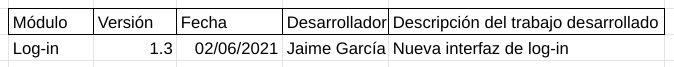
\includegraphics[height=1.3cm]{../images/tabla_versionado_code.png}
    \caption{Tabla de versionado del código.}
    \label{tablaVersionado}
\end{figure}

\begin{figure}[H]
    \centering
        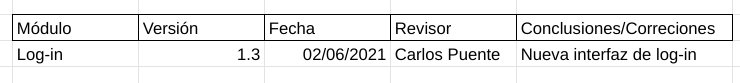
\includegraphics[height=1.5cm]{../images/tabla_conclusiones_revision_pares.png}
    \caption{Tabla de conclusiones de revisión por pares de código.}
    \label{tablaConclusionesPares}
\end{figure}

\textbf{PL.CA.3: Revisión de los requisitos}

Para comprobar el correcto cumplimiento de los requisitos del sistema se utilizará una tabla de cumplimiento de requisitos (figura \ref{tablaRequisitos}). En este tipo de revisión tanto el desarrollador como el revisor rellenarán dicha tabla y discutirán los resultados. Dichos resultados serán recogidos en una tabla de resumen (figura \ref{tablaConclusionesRequisitos}) que servirá como para futuras revisiones. Los módulos de software a desarrollar anteriormente van asociados a ciertos requisitos del sistema. Antes de comenzar el desarrollo de un módulo se concretarán los requisitos finales a los que hace referencia y se generará la plantilla de la tabla de adecuación de requisitos. Como en el modelo de revisión anterior, cuando el desarrollador del módulo termine una versión importante o realice un avance crítico solicitará una revisión al gestor del proyecto este le asignará un revisor adecuado para la tarea. 

\begin{figure}[H]
    \centering
        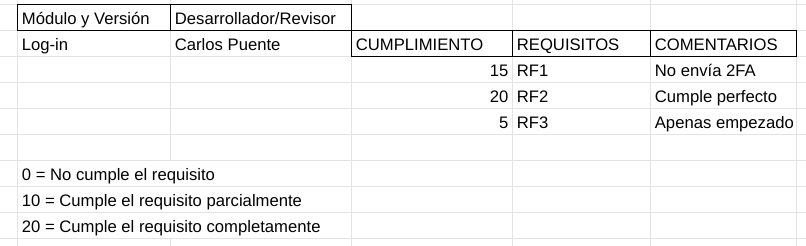
\includegraphics[height=4cm]{../images/tabla_cumplimiento_requisitos.png}
    \caption{Tabla de cumplimiento de requisitos.}
    \label{tablaRequisitos}
\end{figure}

\begin{figure}[H]
    \centering
        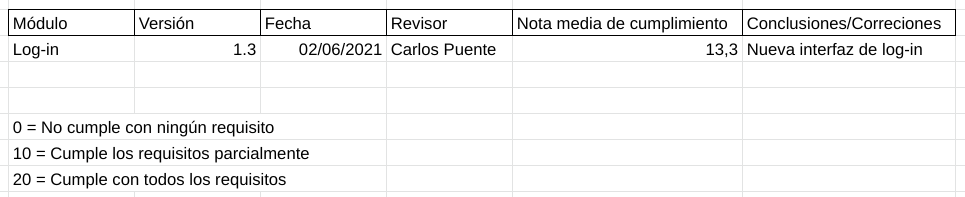
\includegraphics[height=3cm]{../images/tabla_conclusiones_revision_requisitos.png}
    \caption{Tabla de conclusiones de revisión de cumplimiento de requisitos.}
    \label{tablaConclusionesRequisitos}
\end{figure}

Todas estas tablas generadas por el proceso de aseguramiento de la calidad quedarán almacenadas en un directorio remoto accesible por todos los miembros del equipo de desarrollo agrupadas por el módulo al que hacen referencia de manera que sirvan como histórico de las revisiones realizadas y como mecanismo de monitorización del progreso de las tareas.

\textbf{PL.CA.4: Test sobre el producto}

Para asegurar el funcionamiento correcto del código desarrollado se realizarán pruebas de desarrollo sobre los módulos, las cuales consistirán en pruebas unitarias y pruebas de integración con el resto de componentes del sistema. Además, una vez el sistema sea funcional, se realizarán pruebas globales sobre el sistema, las cuales consistirán en pruebas funcionales, de comunicación, de rendimiento, de sobrecarga… etc. Por último, utilizando las herramientas de despliegue continuo mencionadas anteriormente, se implementarán tests básicos 
sobre el sistema previos al despliegue.

\pagebreak

\subsubsection{Calendario del proyecto y división del trabajo}

La división del trabajo se consiste en la partición del trabajo en los siguientes módulos:

Módulo de gestión de \textit{sign-ups} de usuarios, módulo de gestión de log-ins de usuarios, módulo de gestión del Two-Factor-Authentication, módulo de generación de contraseñas, módulo de ranking de robustez de contraseñas, módulo de almacenamiento de contraseñas e información por usuario, módulo de búsqueda y ordenación de contraseñas y módulo de gestión y actualización de contraseñas e información. La documentación será del proyecto será actualizada por cada grupo de trabajo usando las \textit{Wikis} de GitHub después de cada sesión de trabajo, del tal manera que los avances realizados en el desarrollo queden registrados haciendo posible el seguimiento del desarrollo al resto del equipo. El diseño gráfico será realizado por todos los miembros del equipo mediante la creación de un \textit{mockup} de la misma en una reunión conjunta. Las instalaciones y los despliegues serán automáticos y continuos mediante \textit{scripts} de GitHub Actions. Las pruebas (Pruebas de desarrollo sobre los módulos y pruebas globales sobre el sistema) se realizarán conforme los desarrolladores vayan terminando sus designaciones y serán los mismos desarrolladores los cuales pasarán las pruebas, en el punto \ref{sec:calidad} se explica en detalle este aspecto. 

En la operativa diaria se mantendrá un registro del progreso utilizando la herramienta Trello. Se llevará control sobre las tareas pendientes, en curso y completadas.

Se presenta en la figura \ref{gantt-2} un diagrama de Gantt con el desarrollo previsto del proyecto antes del comienzo de este.

\begin{landscape}
    \begin{figure}[H]
        \centering
        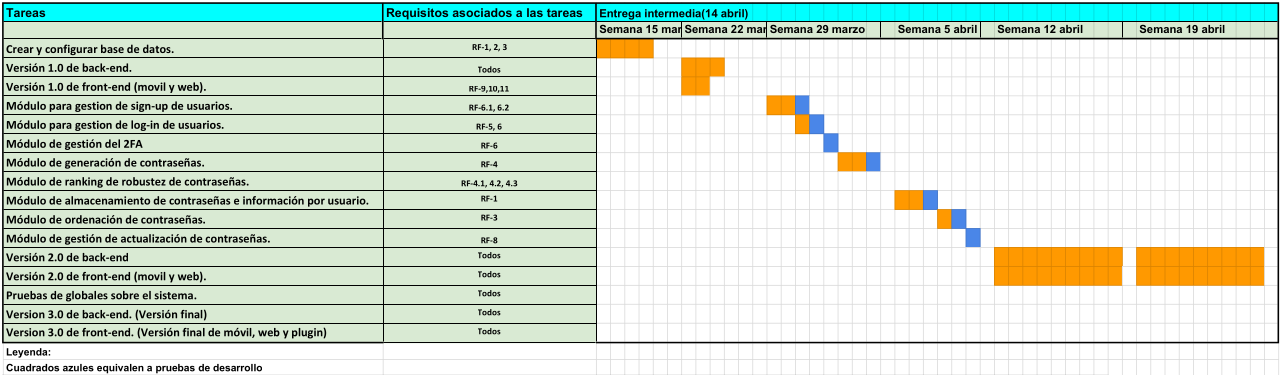
\includegraphics[width=1.4\textheight]{../images/diag-gantt-1.png}
        \label{gantt-1}
    \end{figure}
    
    \begin{figure}[H]
        \centering
        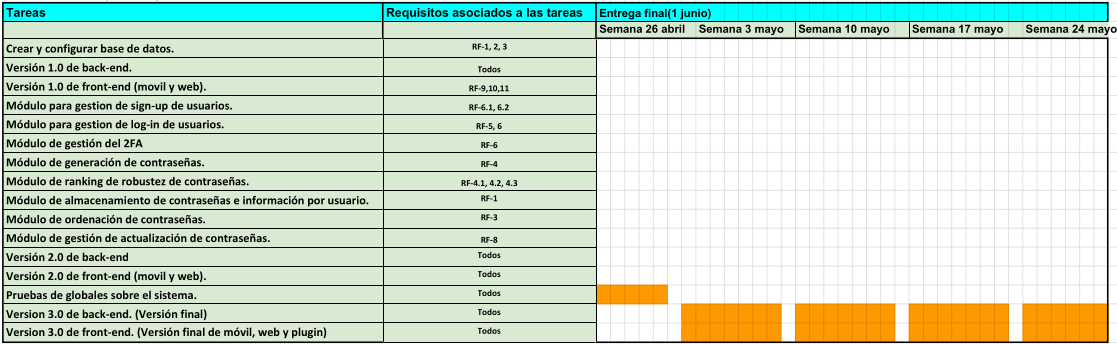
\includegraphics[width=1.4\textheight]{../images/diag-gantt-2.png}
        \caption{Diagrama de Gantt}
        \label{gantt-2}
    \end{figure}
\end{landscape}
    
\section{Análisis y diseño del sistema}

\subsection{Análisis de requisitos}

\begin{table}[H]
    \centering
    \begin{tabular}{| c | p{30em} |}
    \hline
        Código &  Descripción  \\ \hline
        RF-1 & El sistema permite almacenar contraseñas. \\ \hline
        RF-1.1 & El sistema permite almacenar pares que constan de nombre de usuario y contraseña.  \\ \hline
        RF-1.2 & Las entradas de contraseñas tienen un nombre asociado. \\ \hline
        RF-1.3 & El sistema permite asociar a las contraseñas una URL del sitio web al que corresponden. \\ \hline
        RF-1.4 & El sistema registra la fecha de creación o actualización de la contraseña. \\ \hline
        RF-1.5 & El sistema permite almacenar una descripción de texto asociada a la contraseña. \\ \hline
        RF-1.6 & El sistema permite almacenar un único fichero con cualquier extensión asociado a la entrada contraseña. \\ \hline
        RF-1.7 & El sistema permite la creación de contraseñas y la modificación de todos los campos anteriores (nombre, nombre de usuario, contraseña, URL, descripción y fichero). \\ \hline
        RF-2 & El sistema muestra las categorías gestionadas por el usuario. La categoría se define como un directorio donde el usuario almacena contraseñas. Cada contraseña pertenece a una única categoría.\\ \hline
        RF-2.1 & El usuario puede crear, renombrar y eliminar categorías \\ \hline
        RF-3 & El sistema permite visualizar las contraseñas almacenadas\\ \hline
        RF-3.1 & El sistema muestra las contraseñas asociadas a la categoría seleccionada por el usuario. \\ \hline
        RF-3.2 & El sistema muestra los datos y fichero asociados a la contraseña seleccionada. \\ \hline
        RF-3.3 & El sistema permite ordenar las contraseñas de una categoría por fecha de actualización o nombre. \\ \hline
        RF-4 & El sistema permite generación de contraseñas pseudoaleatorias. \\ \hline
        RF-4.1 & El sistema permite seleccionar la longitud de la contraseña a generar.\\ \hline
        RF-4.2 & El sistema permite seleccionar el conjunto de caracteres que compone la contraseña a generar.\\ \hline
        RF-4.3 & El sistema muestra el grado de robustez (entropía) de la contraseña al ser generada. La entropía($E$) se calcula: $E=n\log_2m$. Donde $n$ es la longitud y $m$ el número de caracteres de la población usada.\\ \hline
        RF-5 & El usuario inicia sesión al sistema mediante su correo electrónico y la contraseña maestra. Únicamente podrá acceder con esta contraseña, que no se puede recuperar.\\ \hline
        RF-6 & El sistema requiere 2FA para iniciar sesión. \\ \hline
        RF-6.1 & El sistema permite el registro de un usuario con: correo electrónico, contraseña maestra y un apodo.\\ \hline 
        RF-6.2 & El registro de sesión se deberá confirmar, para verificar la identidad, mediante un correo electrónico a la dirección especificada por el usuario registrado. \\ \hline
        RF-7 & La interfaz de usuario permite copiar al portapapeles del dispositivo la contraseña de una entrada. \\ \hline 
        RF-8 & Se accede al sistema mediante una aplicación para dispositivos móviles Android con versión 6.1 (\textit{Marshmallow}). \\ \hline
        RF-9 & Se accede al sistema mediante una aplicación para navegadores web Google Chrome (versión 89) y Firefox (versión 87). \\ \hline
        RF-10 & El sistema ofrece un \textit{plug-in} para el navegador Google Chrome (versión 89). \\ \hline
    \end{tabular}
\end{table}

\subsection{Diseño del sistema}

\subsubsection*{Diagramas de módulos}

\begin{figure}[H]
    \centering
        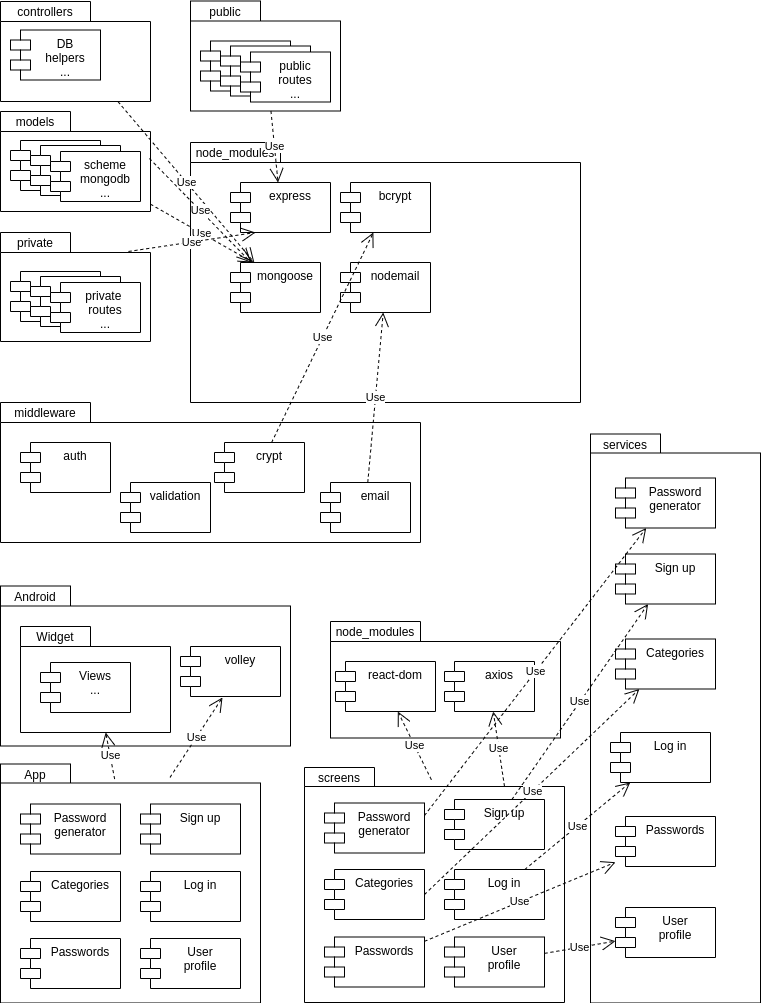
\includegraphics[width=0.99\textwidth]{../images/modulos_v1.png}
    \caption{Diagramas de componentes y conectores.}
    \label{modulos}
\end{figure}
\pagebreak

En el diagrama de módulos en la figura \ref{modulos} se describe las estructuras que el sistema implementa y sus relaciones. Los diferentes paquetes agrupan distintos módulos basándose en su función.

\begin{itemize}
    \setlength{\itemsep}{0em}
    \item 'public': las rutas del modelo accesibles públicamente a través de la API.
    \item 'private': las rutas del modelo que requieren permisos.
    \item 'models': MongoDB \textit{schemes} que modelan la estructura de la información en la base de datos.
    \item 'controllers': colección de módulos que interactúan con la base de datos.
    \item 'middleware': módulos que otorgan funcionalidad variada al sistema.
    \item 'node modules': módulos importados con NPM que ofrecen funcionalidad específica.
    \item 'express': \textit{framework} de desarrollo de servidores web para Node.
    \item 'mongoose': permite la interacción con bases de datos MongoDB.
    \item 'bcrypt': ofrece funcionalidad de cifrado.
    \item 'nodemail': ofrece funcionalidad de envío de correos electrónicos.
    \item 'react-dom': interacción con la vista del navegador web.
    \item 'axios': permite realizar peticiones HTTP al \textit{backend} de la aplicación.
    \item 'screens': vistas del servidor web.
    \item 'services': diferente funcionalidad para la vista de la aplicación.
    \item 'Android': SDK de Android.
    \item 'App': diferentes vistas de la aplicación móvil.
\end{itemize}

Los diferentes módulos externos importados del repositorio de Node o del SDK de Android, ofrecen distinta funcionalidad relativa a las conexiones entre componentes (\textit{e.g. frontend-backend}, \textit{backend}-MongoDB), componentes de vista básicos y seguridad.


\subsubsection*{Diagramas de componentes y conectores}

\begin{figure}[H]
    \centering
        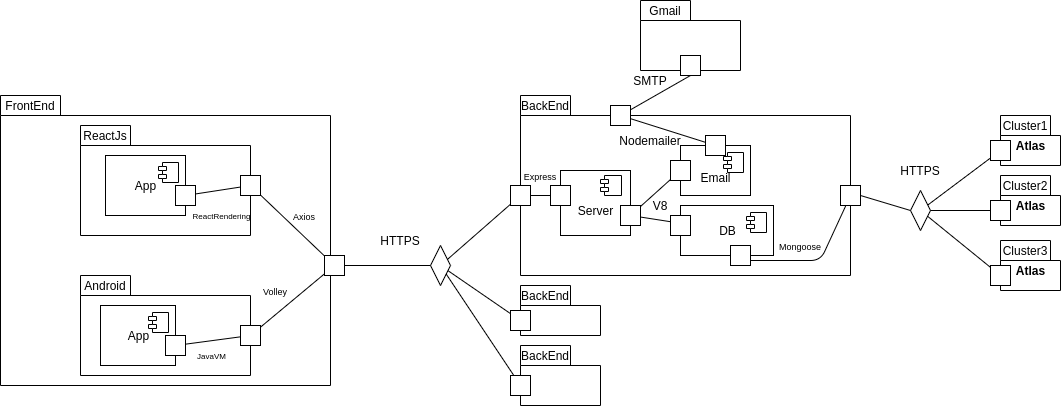
\includegraphics[width=0.90\textwidth]{../images/cyc.png}
    \caption{Diagramas de componentes y conectores.}
    \label{cyc}
\end{figure}

En el diagrama de componentes y conectores en la figura \ref{cyc} se muestra una visión general del sistema, existen tres componentes principales en la aplicación que se relaciona cada uno con una capa del modelo, estos componentes muestran los elementos de presencia en tiempo de ejecución del sistema.

El \textit{frontend} es el componente de la aplicación con el cual el usuario interactúa con el sistema, la aplicación al ser orientada a varias plataformas usa distintos subcomponentes para darle forma a la aplicación, en concreto React.JS, se comunica con el resto de la aplicación mediante el conector React Rendering, De la misma forma lo hace la parte de Android mediante Java Virtual Machine, ambos interaccionan con el resto del sistema usando los puertos que proporcionan las librerías de Axios o Volley.

El conector que relaciona este componente con el componente del \textit{backend} es el protocolo HTTPS a una réplica del servidor.

La interacción entre los componentes de \textit{backend}, es en este caso más compleja el puerto que atiende peticiones utiliza Express, y se comunica con los otros componentes usando el motor V8 como conector, que compila en tiempo de ejecución todos los módulos de JavaScript de la parte del servidor. El sistema a su vez tiene un servidor mail que se comunica mediante el protocolo SMTP y que usa la librería Nodemailer para conectar con Gmail. Por último mantendrá una conexión, también usando el protocolo HTTPS, con la base de datos que se encontrará replicada en varios clústeres y alojada en \textit{MongoDB Atlas}, se usa Mongoose para gestionar la conexión con la base de datos.
% Explicar Interfaces de componentes

% Protocolos de comunicación entre componentes

\subsubsection*{Diagrama de distribución}

\begin{figure}[H]
    \centering
        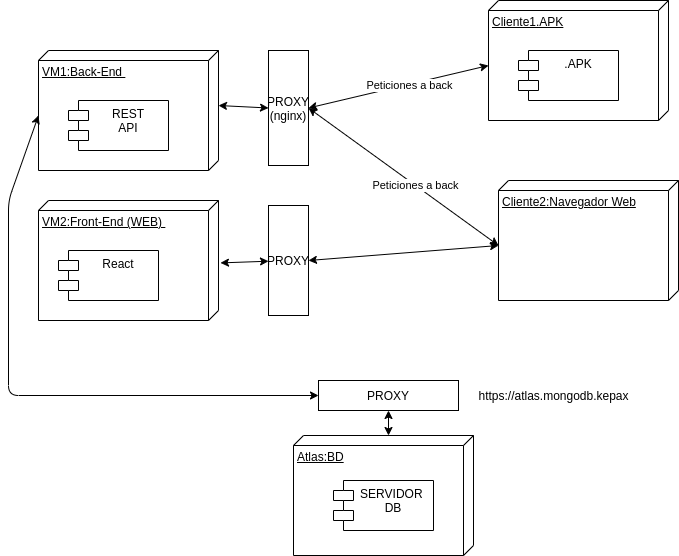
\includegraphics[width=0.99\textwidth]{../images/despliegue.png}
    \caption{Diagrama de distribución.}
    \label{despliegue}
\end{figure}

En el diagrama de despliegue de la figura \ref{despliegue}, se muestra una vista general del sistema en funcionamiento y cómo está distribuido en la nube, en esta vista se asigna cada componente del sistema a un hardware específico.

Tanto el servidor web como el servidor API, se sitúan alojados en los servicios de Amazon AWS y la base de datos se encuentra replicada utilizando MongoDB Atlas.

Se diferencia dos tipos de cliente, el que accede desde un dispositivo móvil y el que accede mediante un protocolo web. El cliente móvil ya tiene compilado el sistema en un dispositivo Android por lo que la capa de acceso a la aplicación este solo tendrá que realizar peticiones directamente a la API REST, a diferencia que el cliente que se conecta mediante un protocolo web, que tendrá en primer lugar que obtener el \textit{template} desde un servidor web para poder realizar peticiones a la API REST.

El servidor cuando requiera realizar operaciones sobre datos persistentes, opera conectándose a un clúster con una réplica de la base de datos MongoDB.

\pagebreak

\subsubsection*{Patrones de diseño y estilos arquitecturales}

A diferencia de la mayoría de \textit{frameworks} que usan el patrón arquitectural modelo vista controlador para separar la lógica de la aplicación de la lógica de vistas, React.JS al ser un \textit{framework} moderno que ofrece \textit{server-side-rendering} por lo que no se puede considerar una arquitectura MVC.
 
La arquitectura usada (figura \ref{patron}) consiste en tres capas con interfaz web, capa de presentación, capa de negocio y capa datos.

\begin{figure}[H]
    \centering
        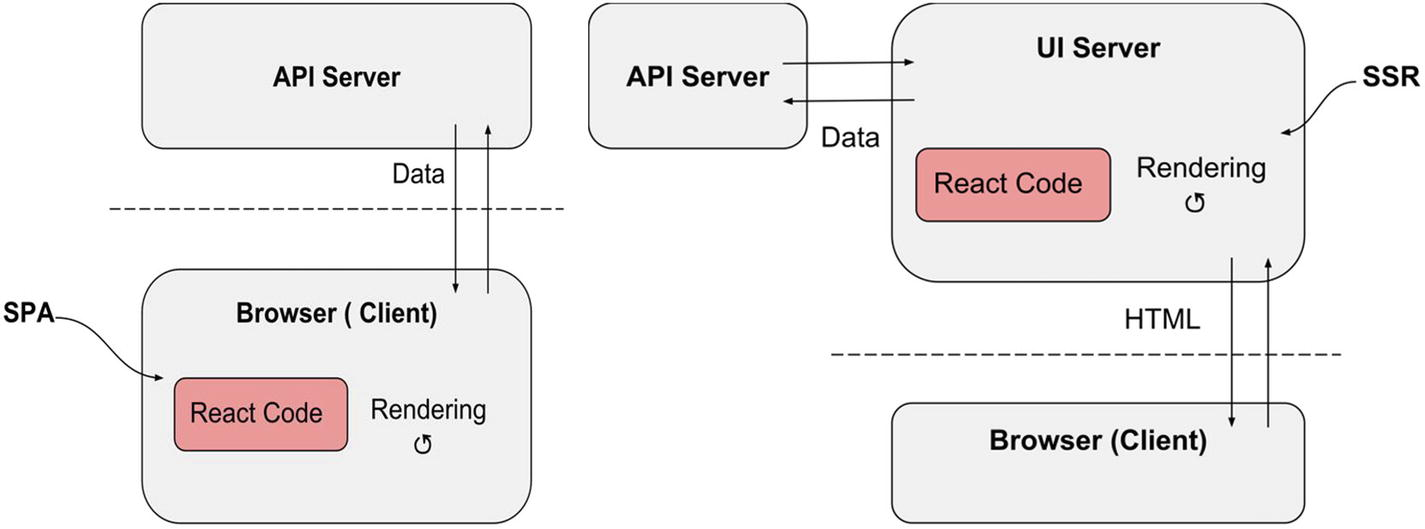
\includegraphics[width=0.99\textwidth]{../images/patron.jpg}
    \caption{Modelo tres capas.}
    \label{patron}
\end{figure}

Como se viene diciendo la capa de presentación o capa de usuario es la que muestra el sistema, le comunica y captura información a la capa de negocio, en esta capa se presentan dos tecnologías Android y React.JS.
 
La capa de negocio es donde se ejecutan las peticiones del usuario y se envían las respuestas de la ejecución, esta capa se comunica con la capa de presentación para atender a las peticiones y con la capa de datos para almacenar o recuperar datos. Para esta capa se utilizará el entorno de ejecución Node.
 
La capa de datos es la encargada de almacenar los datos mediante en gestor de base de datos, en el caso de la aplicación se utiliza la base de datos no relacional MongoDB.


\subsubsection*{Tecnologías elegidas}

Se hará uso de lenguajes de programación como JavaScript para la interfaz web (React) y para el modelo (Node). Es la tecnología requerida por el \textit{stack} de lenguajes para aplicaciones web MERN. Es sencillo, debido a su conocimiento previo, y unifica la tecnología para el desarrollo \textit{backend} y \textit{frontend}.

La aplicación móvil se desarrollará en Java (Android), que permite desarrollo nativo para teléfonos, es ampliamente utilizado y se conoce de proyectos anteriores. Se propuso el uso del entorno React Native, pero se descartó debido a su desconocimiento por parte del grupo.

El componente la vista de la aplicación se conecta a la API de del modelo para realizar peticiones relativas a la acción del usuario. Esta segunda conecta con la base de datos MongoDB en los servidores Atlas de Mongo. Se prefiere el uso de Atlas frente al despliegue de la base de datos en una máquina virtual debido a su facilidad de administración y la disponibilidad ofrecida. 

\pagebreak

La base de datos MongoDb es NoSQL y, frente a una base de datos SQL como Oracle, permite más flexibilidad para recoger y persistir información. Además, MongoDB junto a Mongoose, ofrecen facilidad de interacción con JavaScript mediante ficheros JSON.

Para la creación de la API web ofrecida por servidor del modelo, se ha optado por seguir la estructura API REST, que es ampliamente utilizada y fácil de implementar con las tecnologías utilizadas. 

La tecnología Node hace uso de un bucle de eventos el cual permiten la realización de operaciones asíncronas para realizar peticiones en el \textit{background} y recibir respuestas sin necesidad de interrumpir la operativa esperando a esta.

Se ha optado en utilizar el módulo Bcrypt para cifrar los datos de la aplicación y utilizar el protocolo HTTPS para asegurar las comunicaciones. 

\pagebreak

\section{Memoria del proyecto}

\subsection{Inicio del proyecto}

En la identificación y asignación de recursos a utilizar, se ha decidido en base a los conocimientos tecnológicos de cada integrante del grupo y el grado de familiarización con las tecnologías. 

Respecto a los servidores en \textit{cloud} a utilizar para el despliegue del sistema. El criterio de elección se ha basado en el estudio del impacto a nivel global de la empresa, es decir, grado de utilización en el mundo empresarial y la cantidad de servicios ofrecidos gratuitamente. Finalmente, se decide crear una cuenta en AWS, siendo así Amazon el proveedor de \textit{cloud} para el proyecto.

En relación con la base de datos, se ha decidido usar una base no relacional debido al grado de flexibilidad de modelo de datos que ofrece frente al modelo típico relacional. Como SGBD se ha escogido MongoDB. Se ha creado una cuenta en MongoDB Atlas el cual permite crear una base de datos remota accesible
por el sistema.

En cuanto a la formación inicial de los integrantes, se han tenido en cuenta en el reparto de responsabilidades los conocimientos de los desarrolladores, sin embargo, todos los desarrolladores dedicarán tiempo de manera individual en autoformación y documentación sobre las tecnologías a usar en el desarrollo del sistema. Además, todos los integrantes del grupo se han comprometido a formar a sus compañeros en las áreas que conozcan a medida que surjan dudas durante el desarrollo del sistema.

\subsection{Ejecución y control del proyecto}

Las comunicaciones entre los miembros del grupo de trabajo se realizarán principalmente a través de la herramienta de comunicación Whatsapp, mediante la cual se concretan los horarios de trabajo y se informa acerca de actualizaciones puntuales en las tareas asignadas a cada miembro para que todo el equipo quede informado de cómo avanzan los distintos componentes del trabajo. Además, las reuniones semanales de puesta en común del trabajo se realizarán utilizando la herramienta de videoconferencia Google Meet. Esta última será el principal medio de comunicación del grupo. Destacar que pese a la división de trabajo previo, se intenta trabajar de manera conjunta por videoconferencia, de manera que se puedan poner en común y resolver problemas en la medida en que surjan.

En cuanto al registro de las decisiones tomadas en las reuniones, se plasmarán en actas de cada una de ellas. El almacenamiento de estas actas se realizará en un directorio remoto en GitHub.

Partiendo de la división inicial del grupo en equipos de trabajo detallada en el punto 2, los responsables de cada equipo de trabajo se encargarán de monitorizar el avance de sus respectivos módulos, determinar las tareas a realizar, asignar dichas tareas a los desarrolladores y marcar límites temporales y prioridades para cada tarea. En cuanto al trabajo de documentación de los avances sobre el código, todos los desarrolladores serán responsables de registrar los mismos en las \textit{wikis} de GitHub habilitadas para ello en cada repositorio de código. Así mismo, los desarrolladores tendrán que rellenar una tabla de control de esfuerzos para registrar su trabajo y cumplir con el resto de planes especificados más adelante.




\pagebreak

Respecto a la monitorización y control del progreso del proyecto, todas las semanas se realizará una reunión conjunta de control en una hora y día fija a la cual asistirán todos los miembros del grupo para exponer los avances realizados durante la semana y poder determinarse el estado del proyecto y las siguientes tareas a desarrollar. Así mismo, tal y como se detalla en el punto \ref{sec:calidad}, existen mecanismos para asegurar la calidad del producto y detectar posibles de rendimiento en el completado de las tareas.

La entrega de resultados se hará de manera continua de forma que el cliente pueda ir viendo el progreso del proyecto. El equipo se compromete a entregar los resultados del mismo en los plazos preestablecidos. Los resultados finales, que contendrán los códigos fuente, \textit{scripts} de compilación y despliegue, etc. también serán entregados al cliente.

Para implementar las vistas del sistema se utilizará por una parte Java (Android SDK) para construir el cliente móvil para dispositivos Android y por otra JavaScript (React.JS) para desarrollar el \textit{frontend} web. En cuanto al \textit{backend}, se desarrollará utilizando Node.JS y la \textit{framework} Express. La base de datos utilizará el SGBD MongoDB. El despliegue del sistema se realizará en un entorno de contenedores Docker desplegado sobre máquinas virtuales en \textit{cloud}. Se seguirá una filosofía de entrega y despliegue continuo utilizando \textit{scripts} y GitHub Actions.

\subsubsection*{Ejecución de los planes:}



\textbf{PL.G.1:} 
EL plan de nombrado de archivos ha probado ser útil para comprender la disposición del código y asegura la navegabilidad del mismo cumpliendo por tanto su objetivo. Ha sido respetado por todos los desarrolladores, resultando ser intuitivo a la hora de ser utilizado mientras se desarrolla. Como problema podría destacarse que en el entorno de Express ha sido menos intuitivo utilizar la convención de nombrado ya que generalmente los archivos se nombran comenzando por minúscula.

\textbf{PL.G.2:} 
El plan de estructurado de directorios cumplido su objetivo habiendo ayudado a los desarrolladores a mantener una correcta estructura de código en los distintos subproyectos y ayudando a su vez la navegabilidad y comprensión del código.

\textbf{PL.G.3:}
Los desarrolladores del proyecto se han valido de las guías de estilo recomendadas por el plan de uso de guía de estilo, acudiendo a ellas a la hora de implementar código.

\textbf{PL.G.4:}
El plan de control de versionado y actualización del código ha resultado ser muy útil para mantener el cógido accesible por todos desarrolladores. Se destaca que la herramiente GitHub ha permitido a los desarrolladores ver el código del resto de los integrantes del código, asegurar que el código no se pierda, acceder a versiones de código anteriores para comprobar configuraciones anteriores y mantener un régimen de despliegue y entrega continuos. La herramienta y el uso de esta ha sido adoptada por todos los integrantes del proyecto sin ningún problema, destacando todos ellos su facilidad y comodidad de uso.

\textbf{PL.CD.1:}
El sistema se encuentra desplegado en su totalidad sobre dos maquina del servicio de \textit{Amazon Web Services}, y se puede acceder a las rutas de la Rest API solo a través del puerto 443 (puerto https) redirigiendo las peticiones del puerto 80 al 443 para mantener la confidencialidad. Estas peticiones son reexpedidas usando el \textit{reverse proxy} Nginx, para asegurarse una conexión segura el proxy obtiene el certificado digital mediante la entidad certificadora Let 's Encrypt, que proporciona certificados de forma gratuita.
 
Entre las principales desventajas que conlleva usar el servicio gratuito de \textit{Amazon Web Services} es que no ofrece una IP estática para la máquina, por ello se ha tenido que utilizar el servicio gratuito no-ip que proporciona dominios a Ip's de forma dinámica, lo que provee a las máquinas cliente y servidor, de dos nombres DNS por las que se les puede identificar. La máquina servidor(backend) está bajo el nombre del dominio \textit{https://keypax-api.sytes.net} y la maquina cliente(frontend) está bajo el nombre \textit{https://keypax.sytes.net}.

\pagebreak

\textbf{PL.CA.1:}
En el ámbito de planes de aseguramiento de la calidad, el plan de uso de guías de documentacióny de diseño gráfico ha resultado más díficil de aplicar que el resto de planes. En cuando al uso de guía de documentación, los desarrolladores han consultado los estándares del mercado para basarse en ellos a la hora de completar la documentación. Sin embargo se ha escogido documentar el código sin seguir estrictamente dichos estándares y buscando un estilo comprensible por todos los integrantes del proyecto. Respecto a las guías de diseño gráfico, los desarrolladores de los componentes de \textit{Frontend} se han asegurado de diseñar las vistas de usuario de forma que sean claras, simples y fáciles de usar por los usuarios futuros.

\textbf{PL.CA.2:}
El plan de revisión de código por pares ha sido llevado a cabo por los desarrolladores tal y como se había estipulado. Ha resultado ser útil para mantener un control del avance y la calidad del código. Sin embargo, se prevee que su utilidad crezca en la segunda iteración del proyecto a medida que vayan creciendo los registros de las revisiones.

\textbf{PL.CA.3:}
EL plan de revisión de requisitos ha sido llevado a cabo por los desarrolladores tal y como se había estipulado.
Se ha comprobado su utilidad a la hora de mantener el control sobre el avance de los requisitos, asegurando que ningún requisito queda sin implementarse. Sin embargo, se prevee que su utilidad crezca en la segunda iteración del proyecto a medida que vayan creciendo los registros de las revisiones pudiendo comprobarse el avance real del proyecto.

\textbf{PL.CA.4:}
El plan de test sobre el producto ha permitido asegurar la correción de los distintos módulos a la vez que se desarrollaban permitiendo detectar bugs antes de integrarlos con el resto de componentes del systema. En la segunda iteración se desarrollarán las pruebas generales previstas sobre el producto completo.


\subsection{Cierre del proyecto}

\section*{Conclusiones}
\addcontentsline{toc}{section}{Conclusiones}

\section*{Glosario}
\addcontentsline{toc}{section}{Glosario}

\section*{Anexo I. Actas de todas las reuniones realizadas}
\addcontentsline{toc}{section}{Anexo I. Actas de todas las reuniones realizadas}
\begin{figure}
    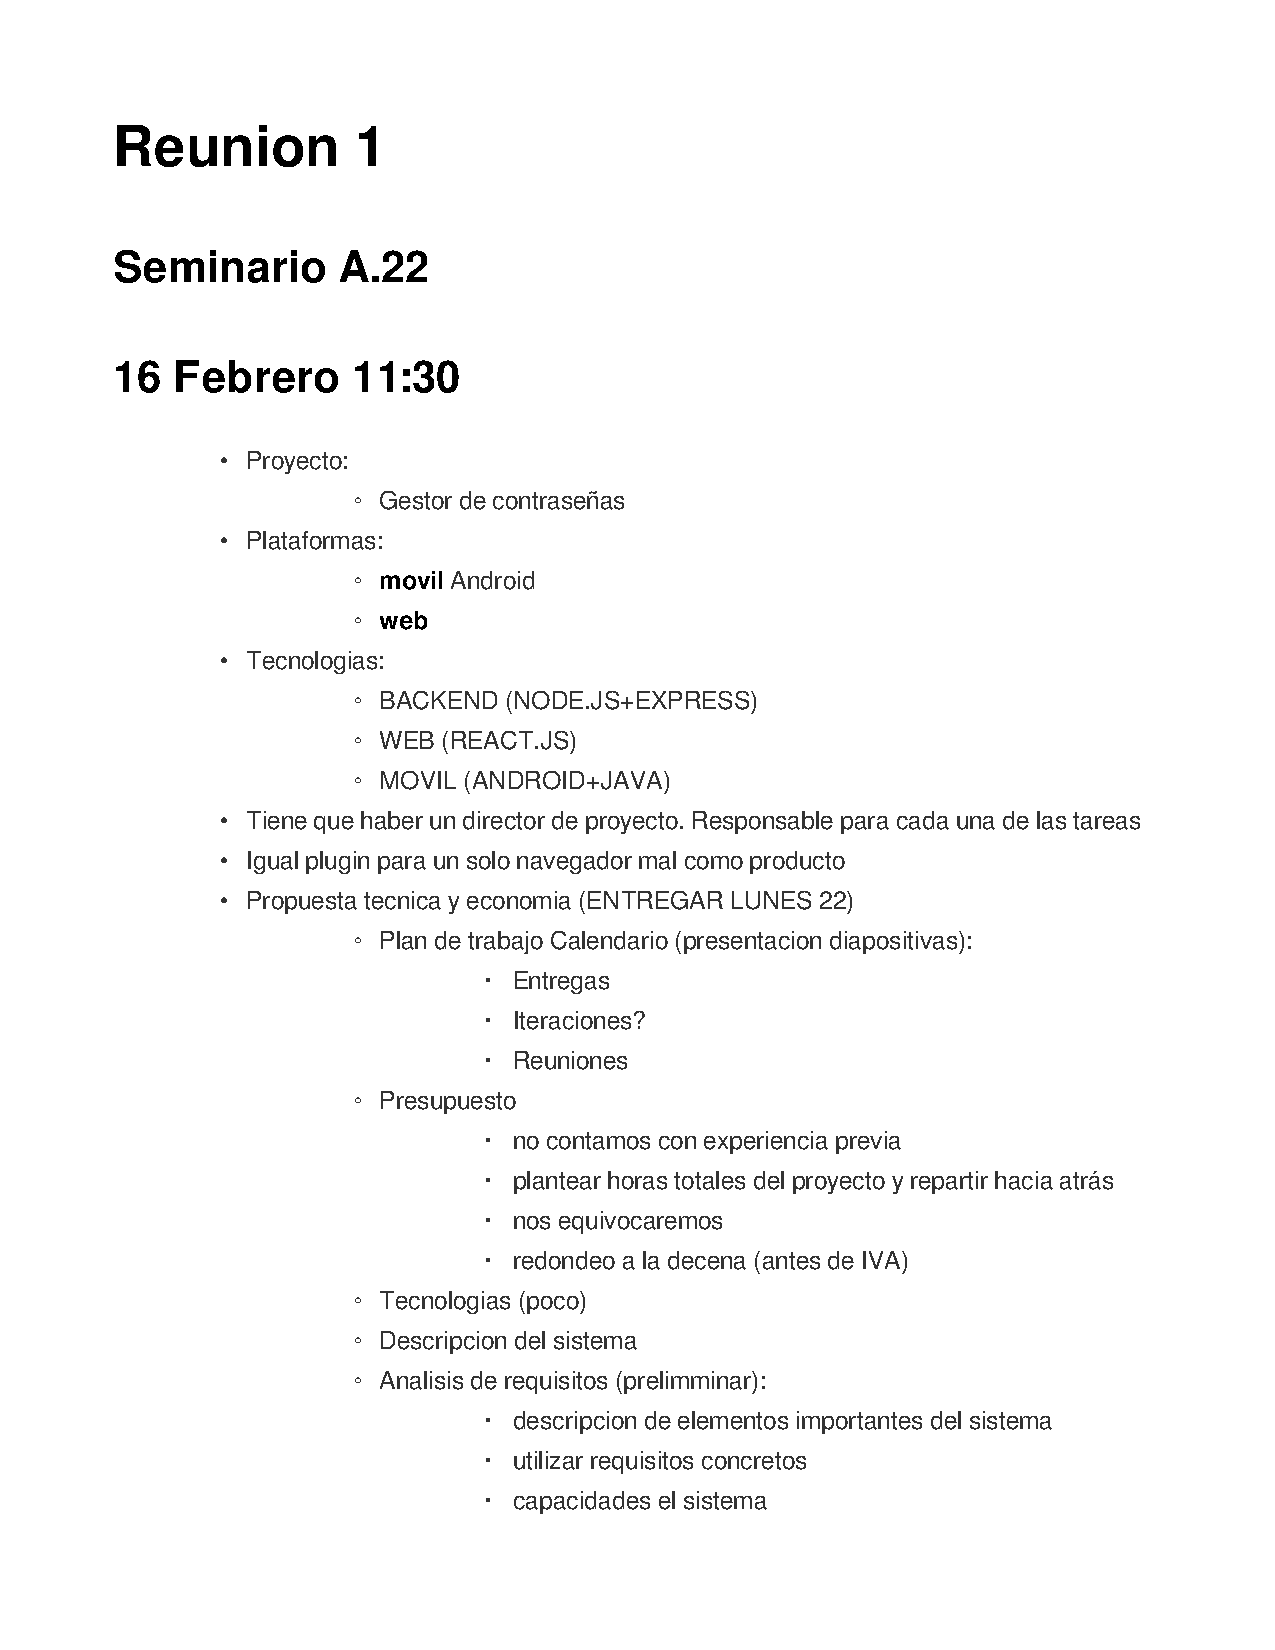
\includegraphics[width=.8\textwidth]{../../actas_reuniones/acta1.pdf}
    \caption{Acta 1}
\end{figure}
\begin{figure}
    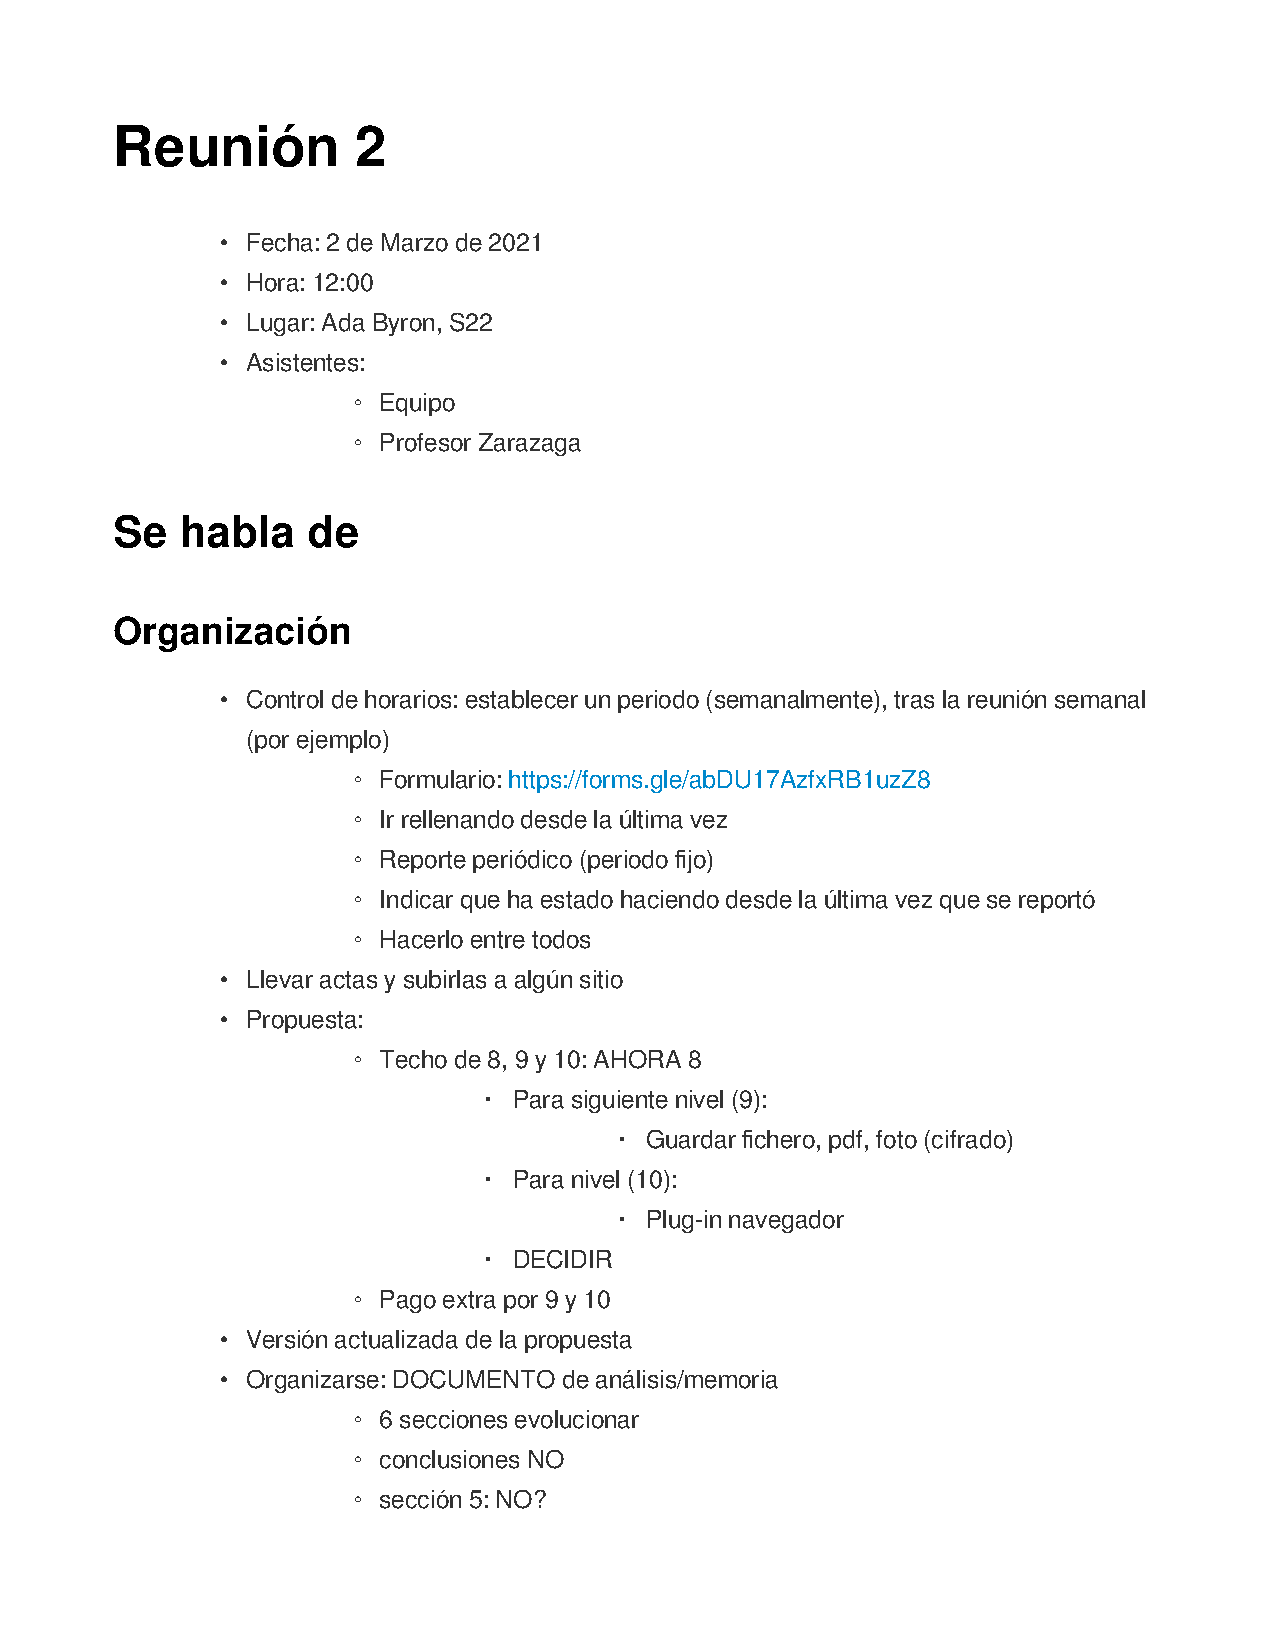
\includegraphics[width=.8\textwidth]{../../actas_reuniones/acta2.pdf}
    \caption{Acta 2}
\end{figure}
\begin{figure}
    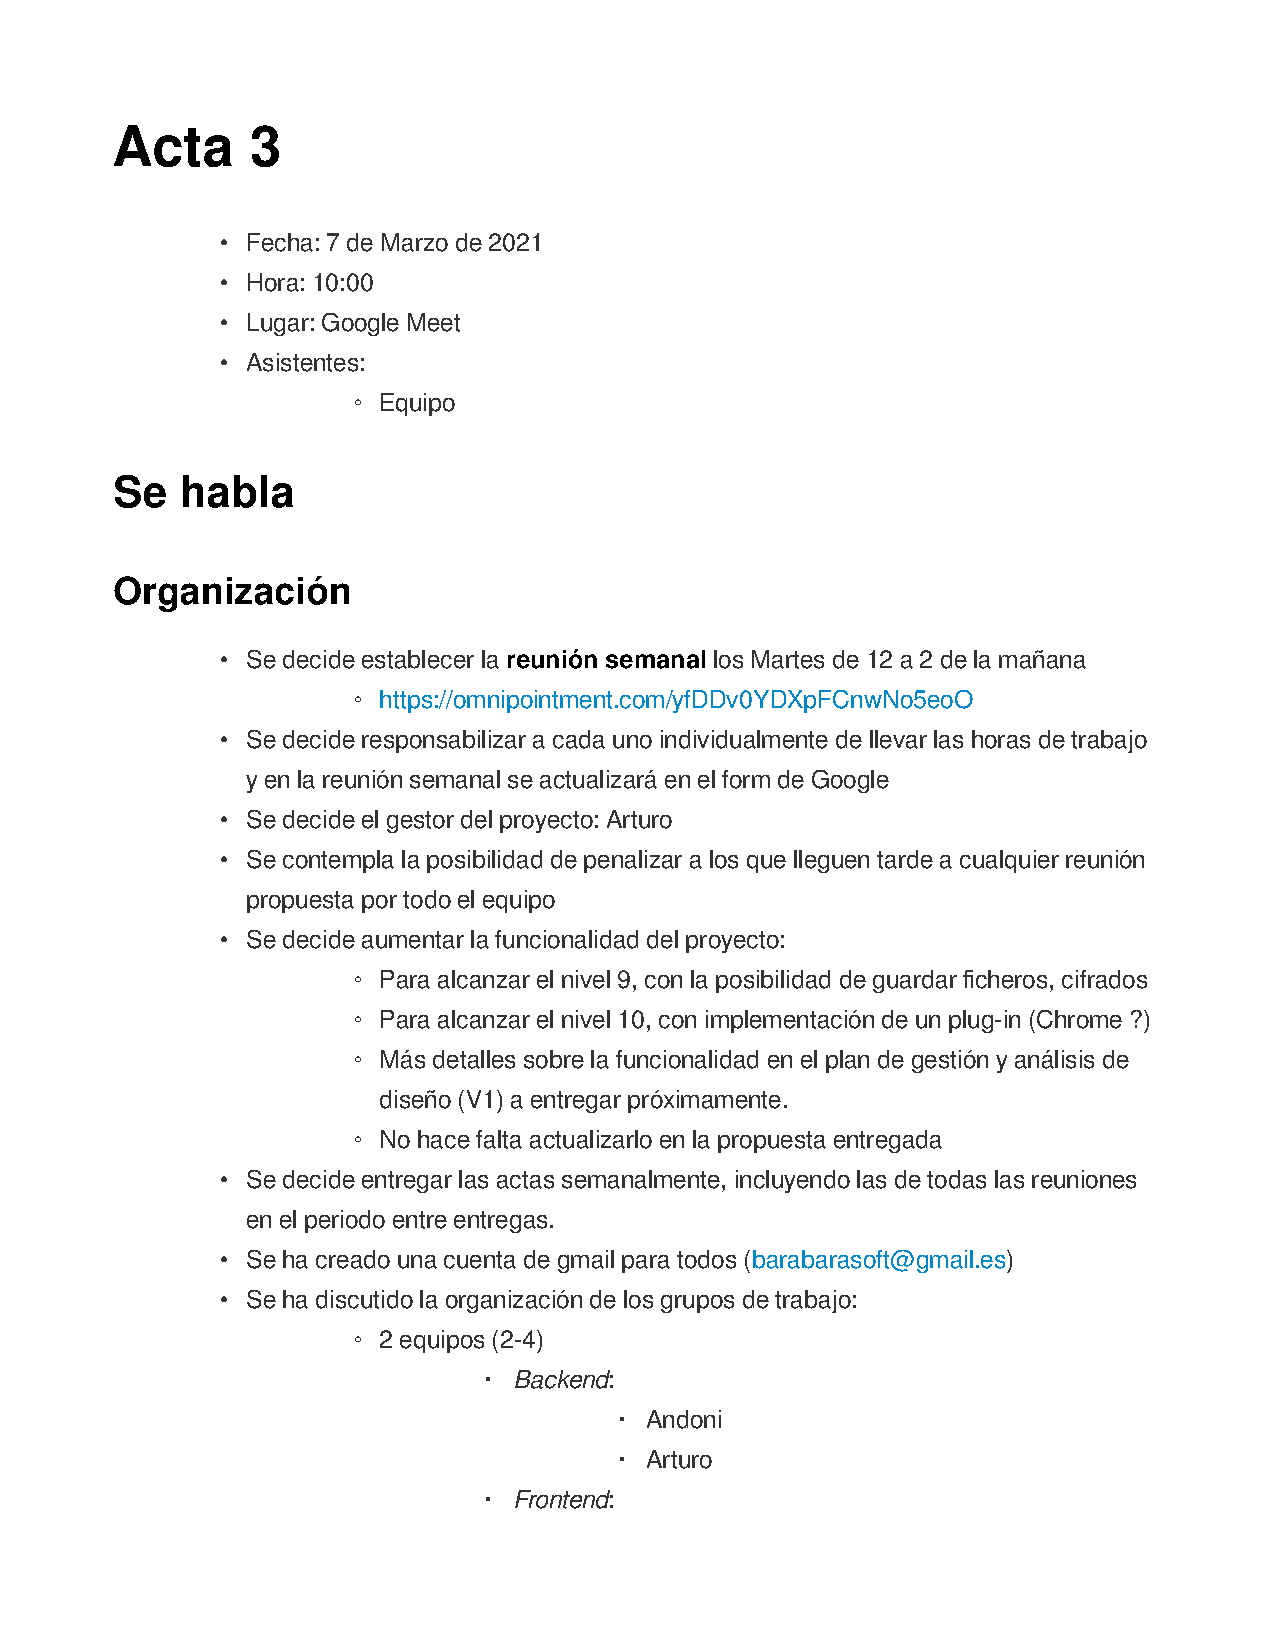
\includegraphics[width=.8\textwidth]{../../actas_reuniones/acta3.pdf}
    \caption{Acta 3}
\end{figure}
\begin{figure}
    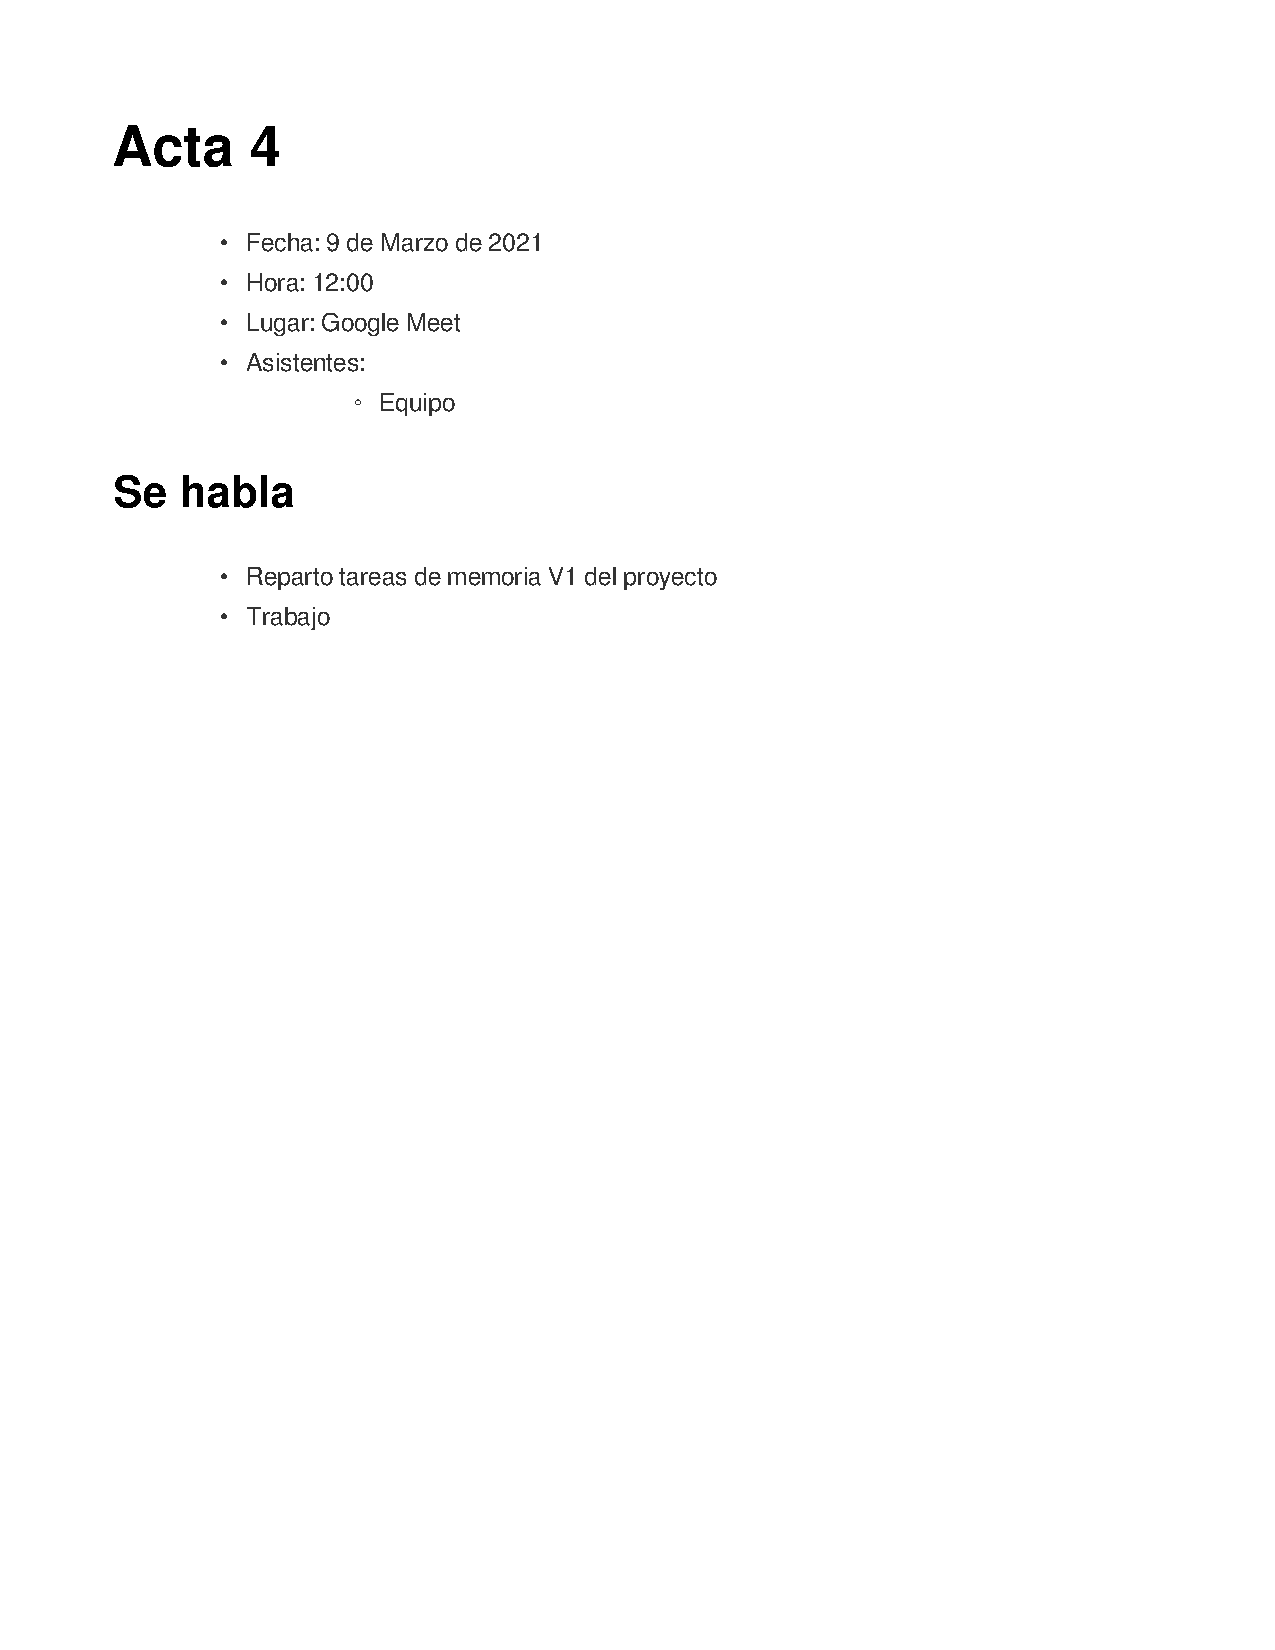
\includegraphics[width=.8\textwidth]{../../actas_reuniones/acta4.pdf}
    \caption{Acta 4}
\end{figure}
\begin{figure}
    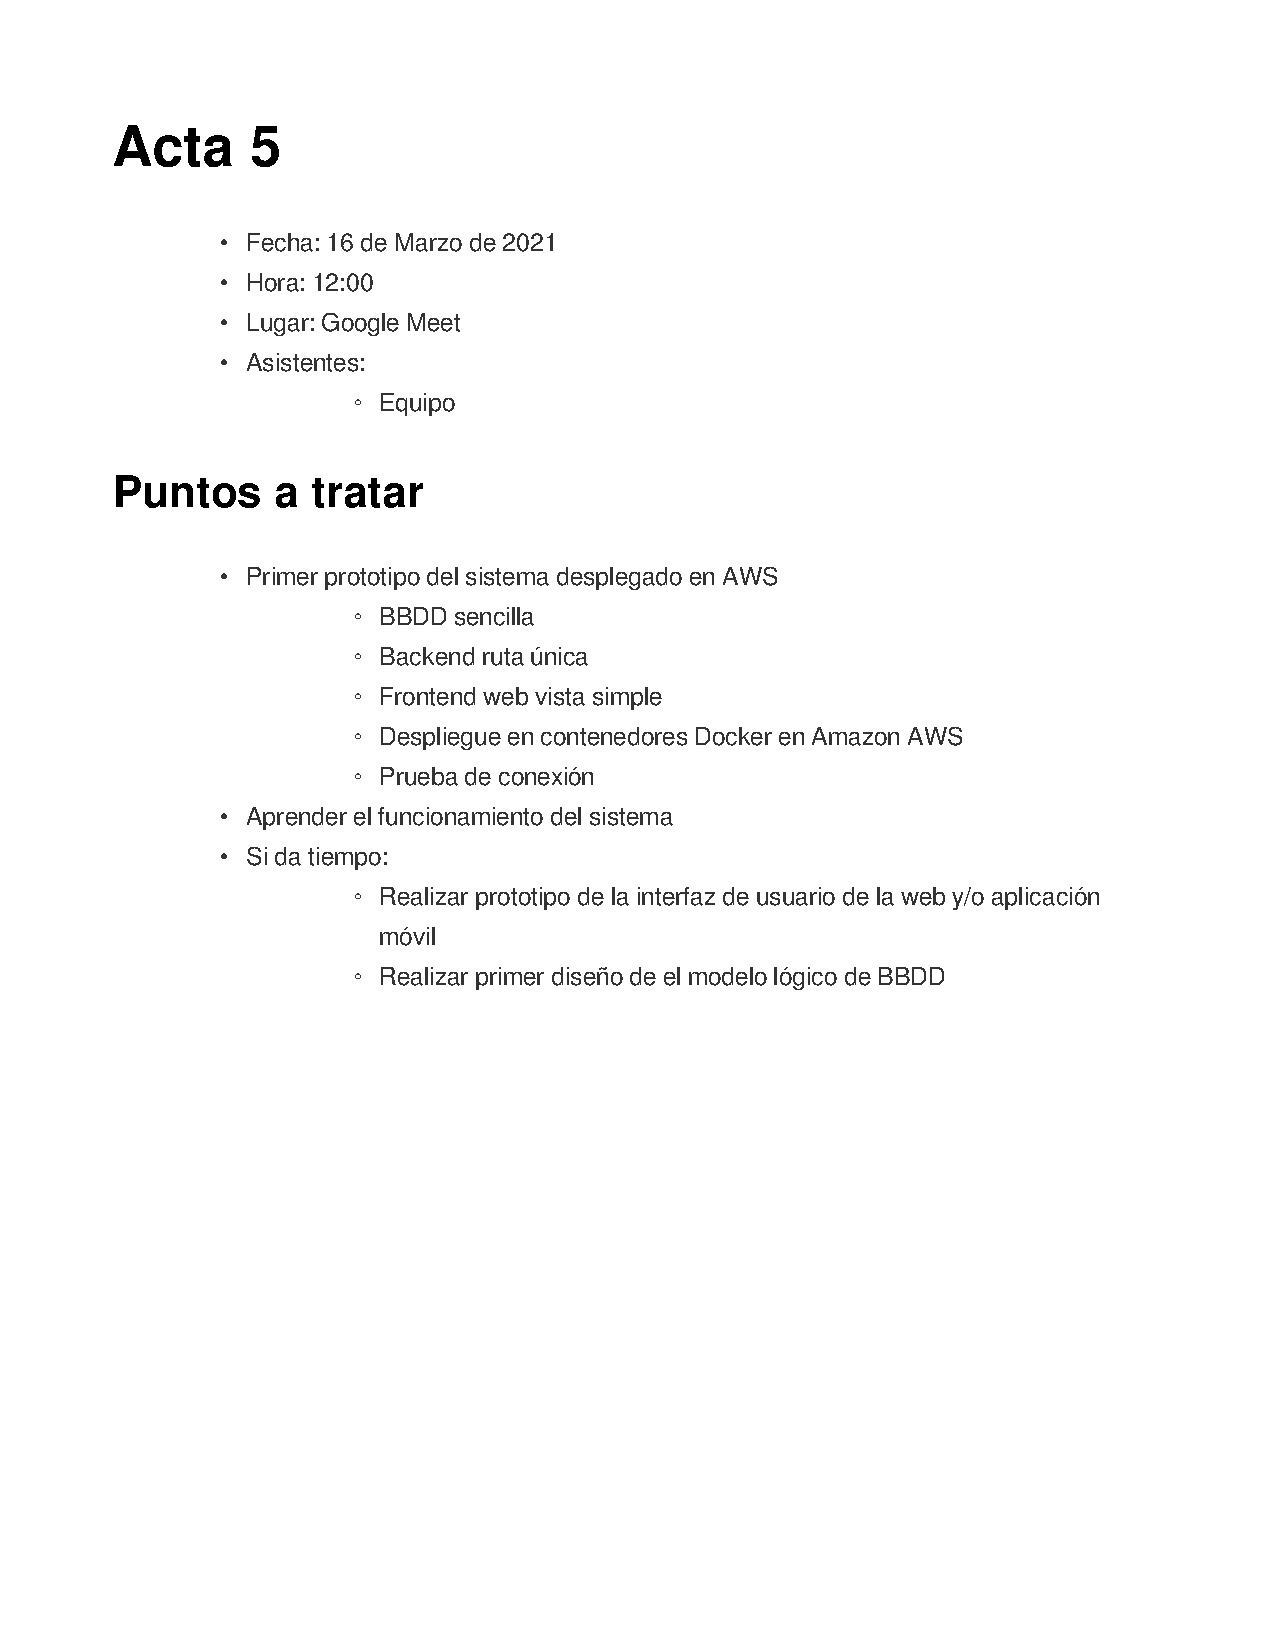
\includegraphics[width=.8\textwidth]{../../actas_reuniones/acta5.pdf}
    \caption{Acta 5}
\end{figure}
\begin{figure}
    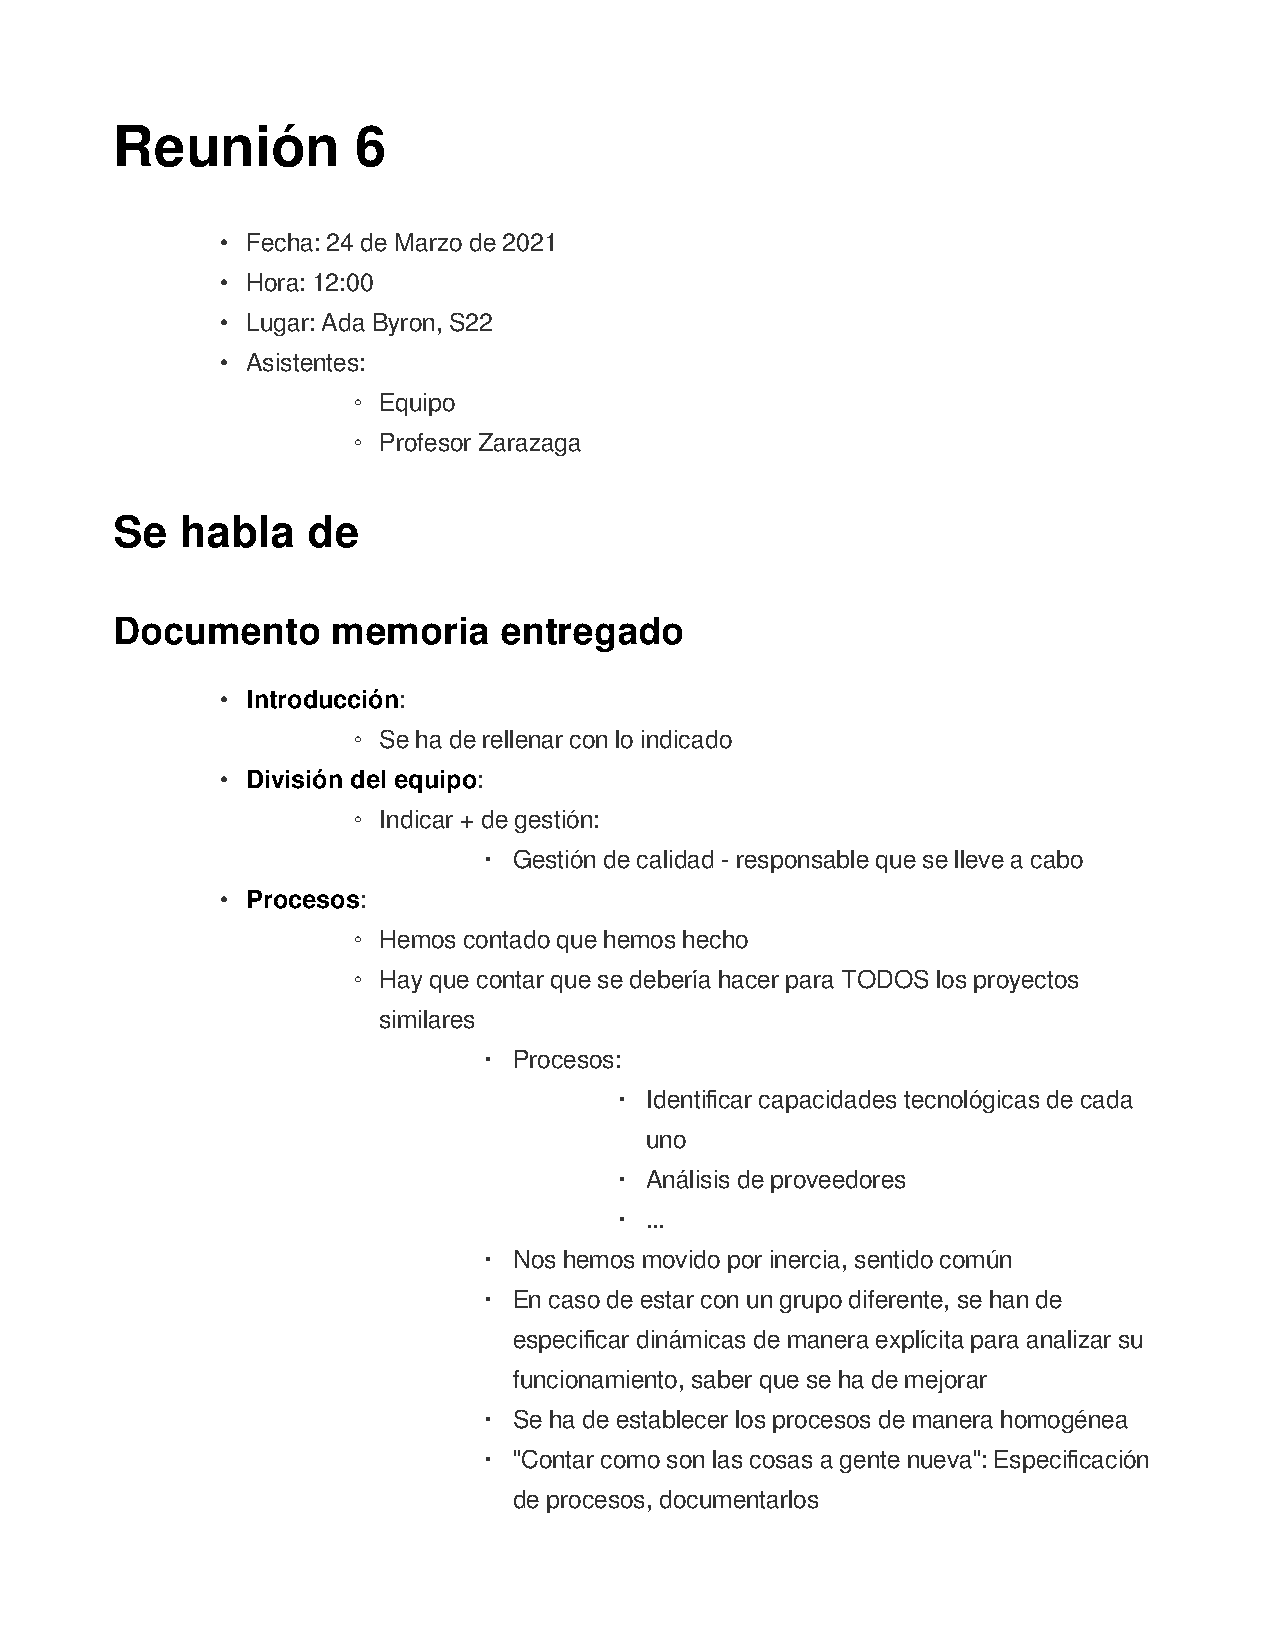
\includegraphics[width=.8\textwidth]{../../actas_reuniones/acta6.pdf}
    \caption{Acta 6}
\end{figure}
\begin{figure}
    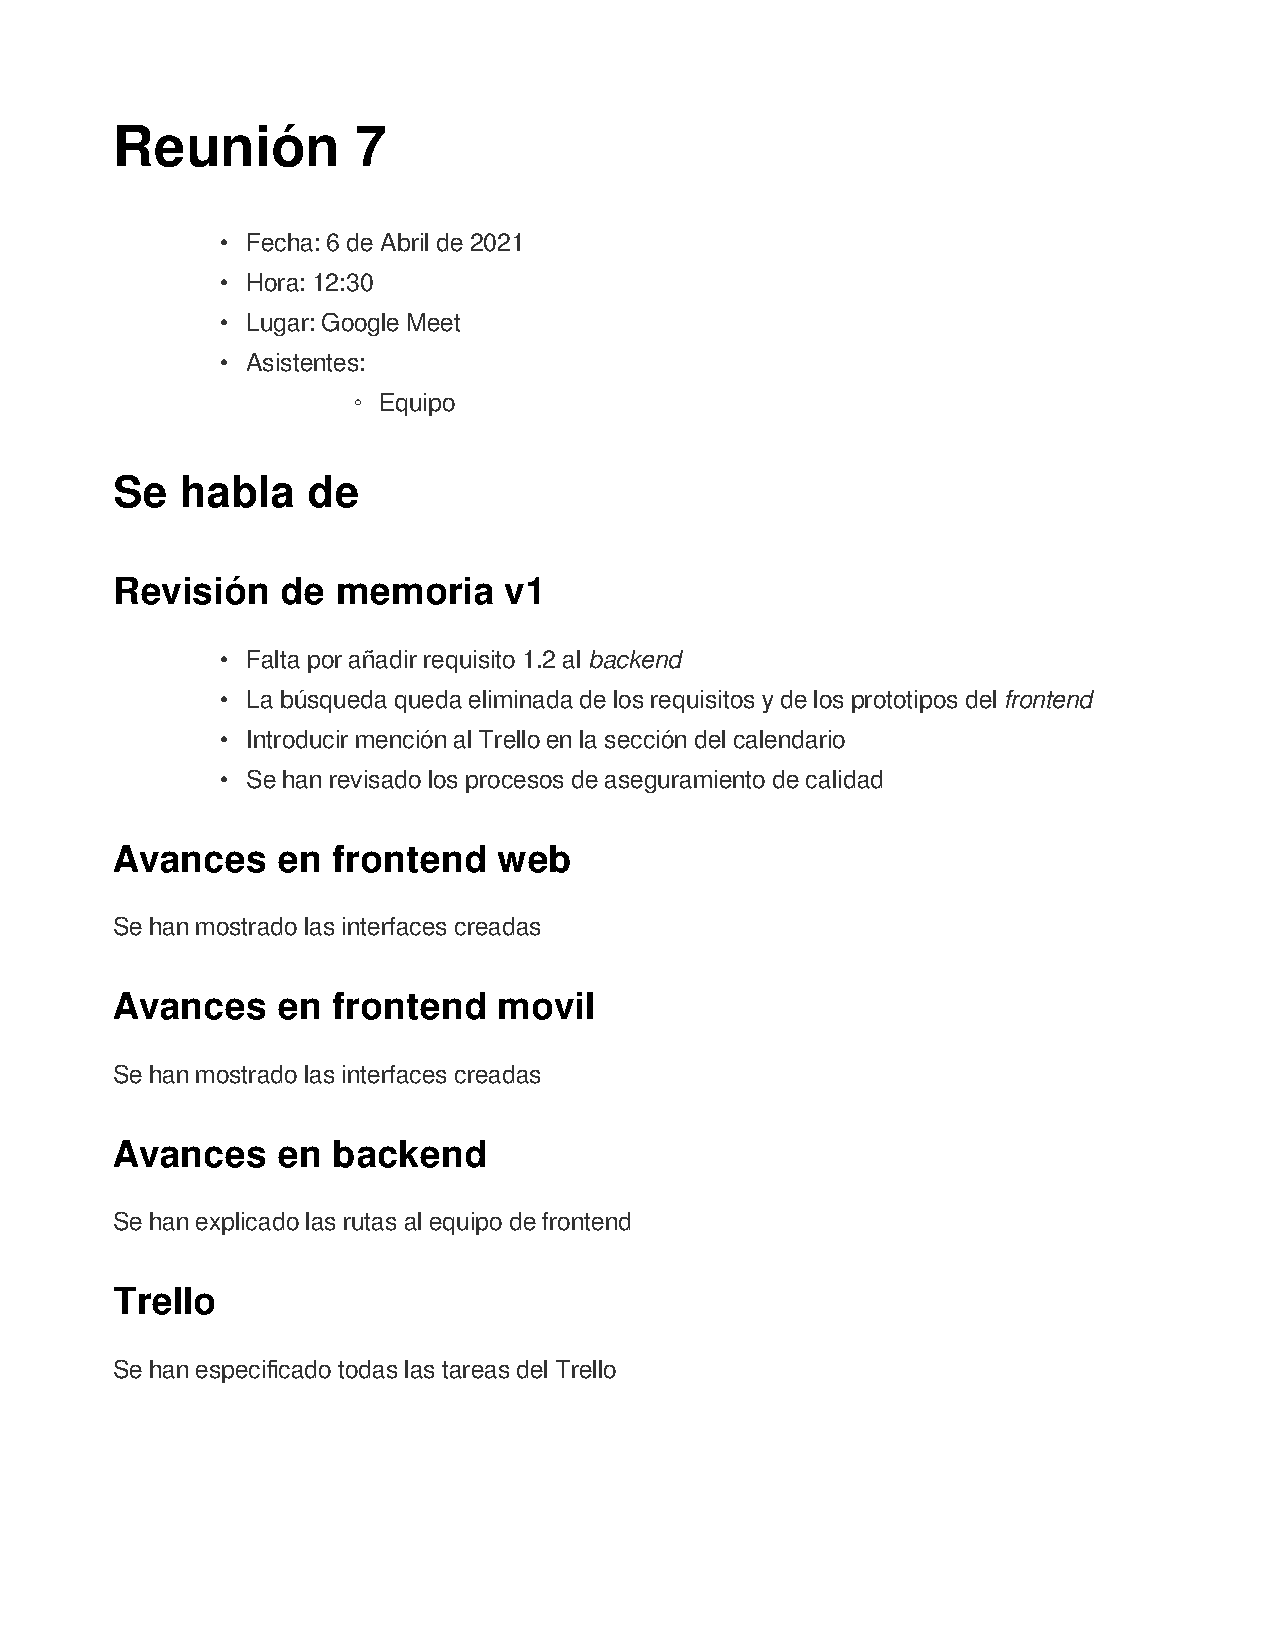
\includegraphics[width=.8\textwidth]{../../actas_reuniones/acta7.pdf}
    \caption{Acta 7}
\end{figure}
\begin{figure}
    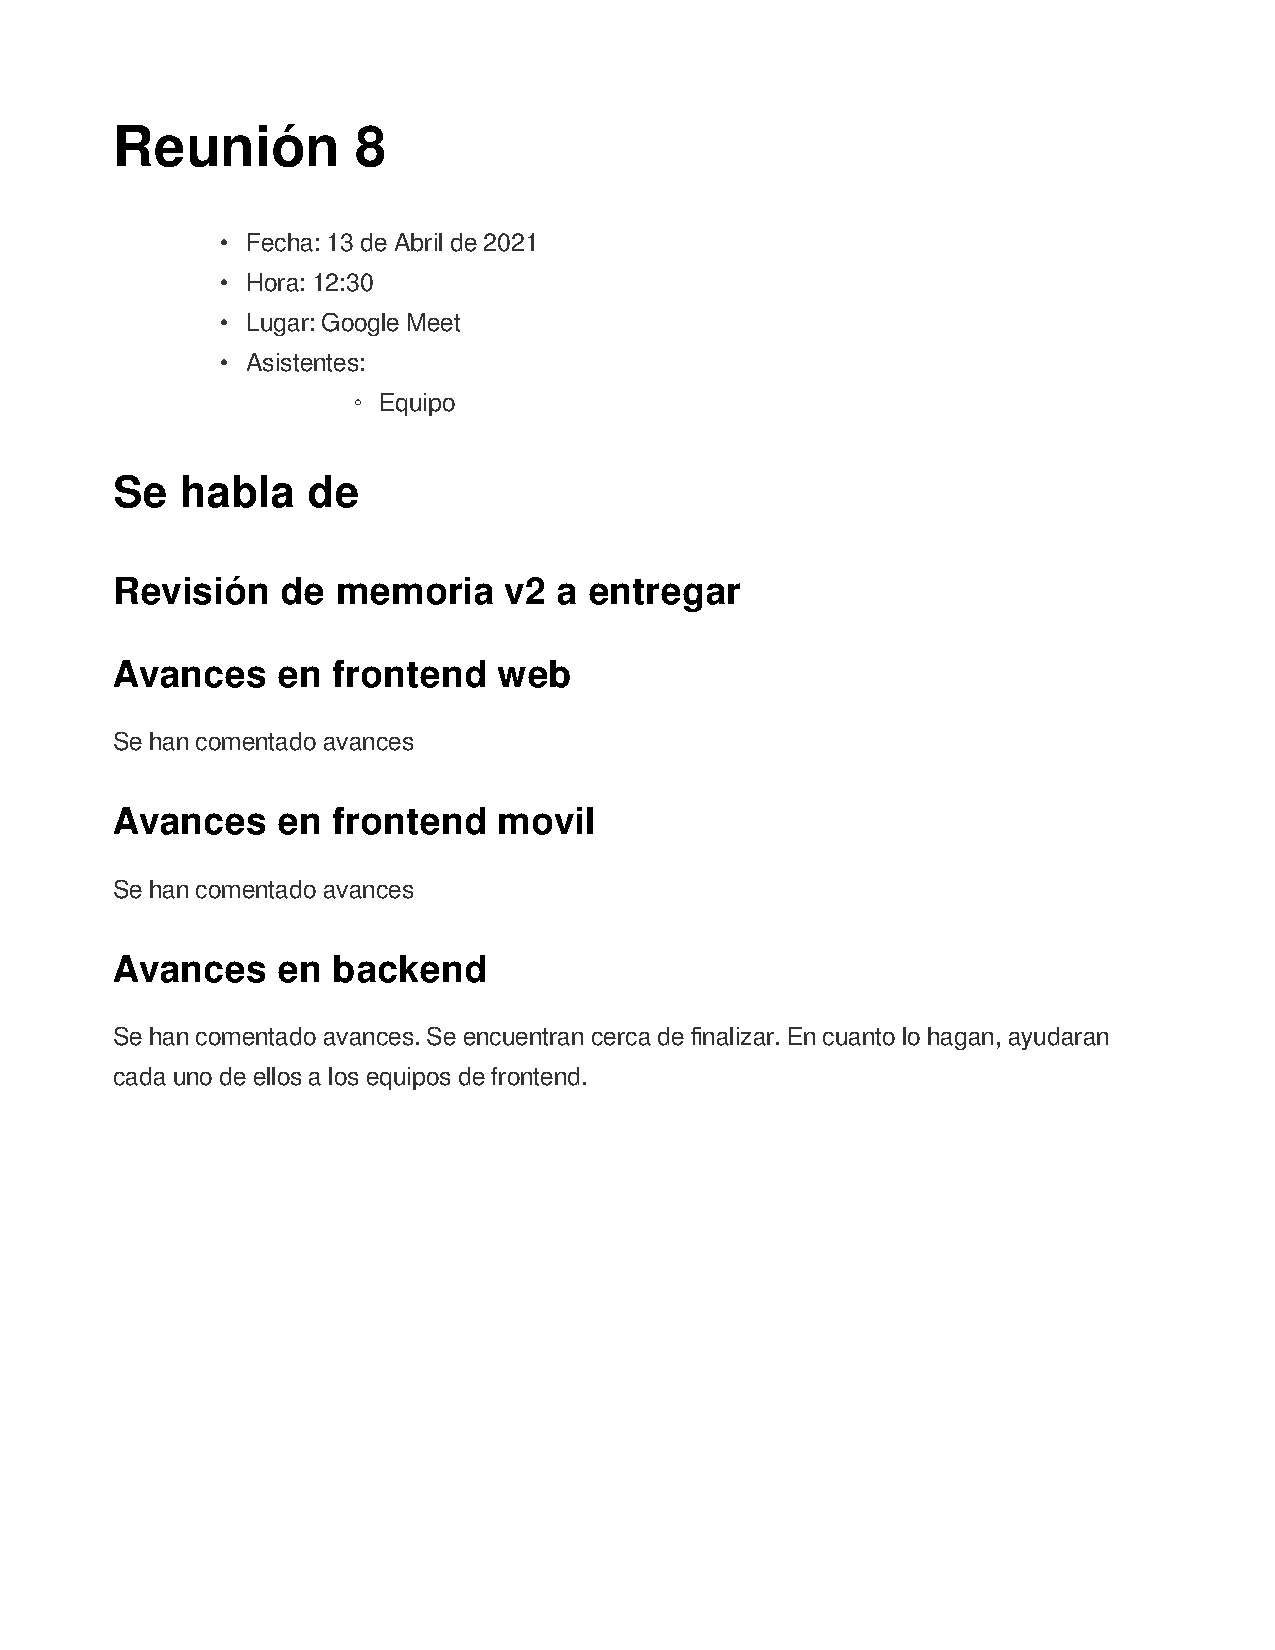
\includegraphics[width=.8\textwidth]{../../actas_reuniones/acta8.pdf}
    \caption{Acta 8}
\end{figure}

\section*{Bibliografía}
\addcontentsline{toc}{section}{Bibliografía}
\end{document}
